\section{Gestion des utilisateurs}

\textbf{Si vous êtes un membre du staff, et que vous avez la permission de gérer les utilisateurs}, vous pouvez alors accéder à la page de gestion des utilisateurs, depuis l'onglet \enquote{Staff} tout à droite du menu de navigation.

\begin{figure}[H]
\centering
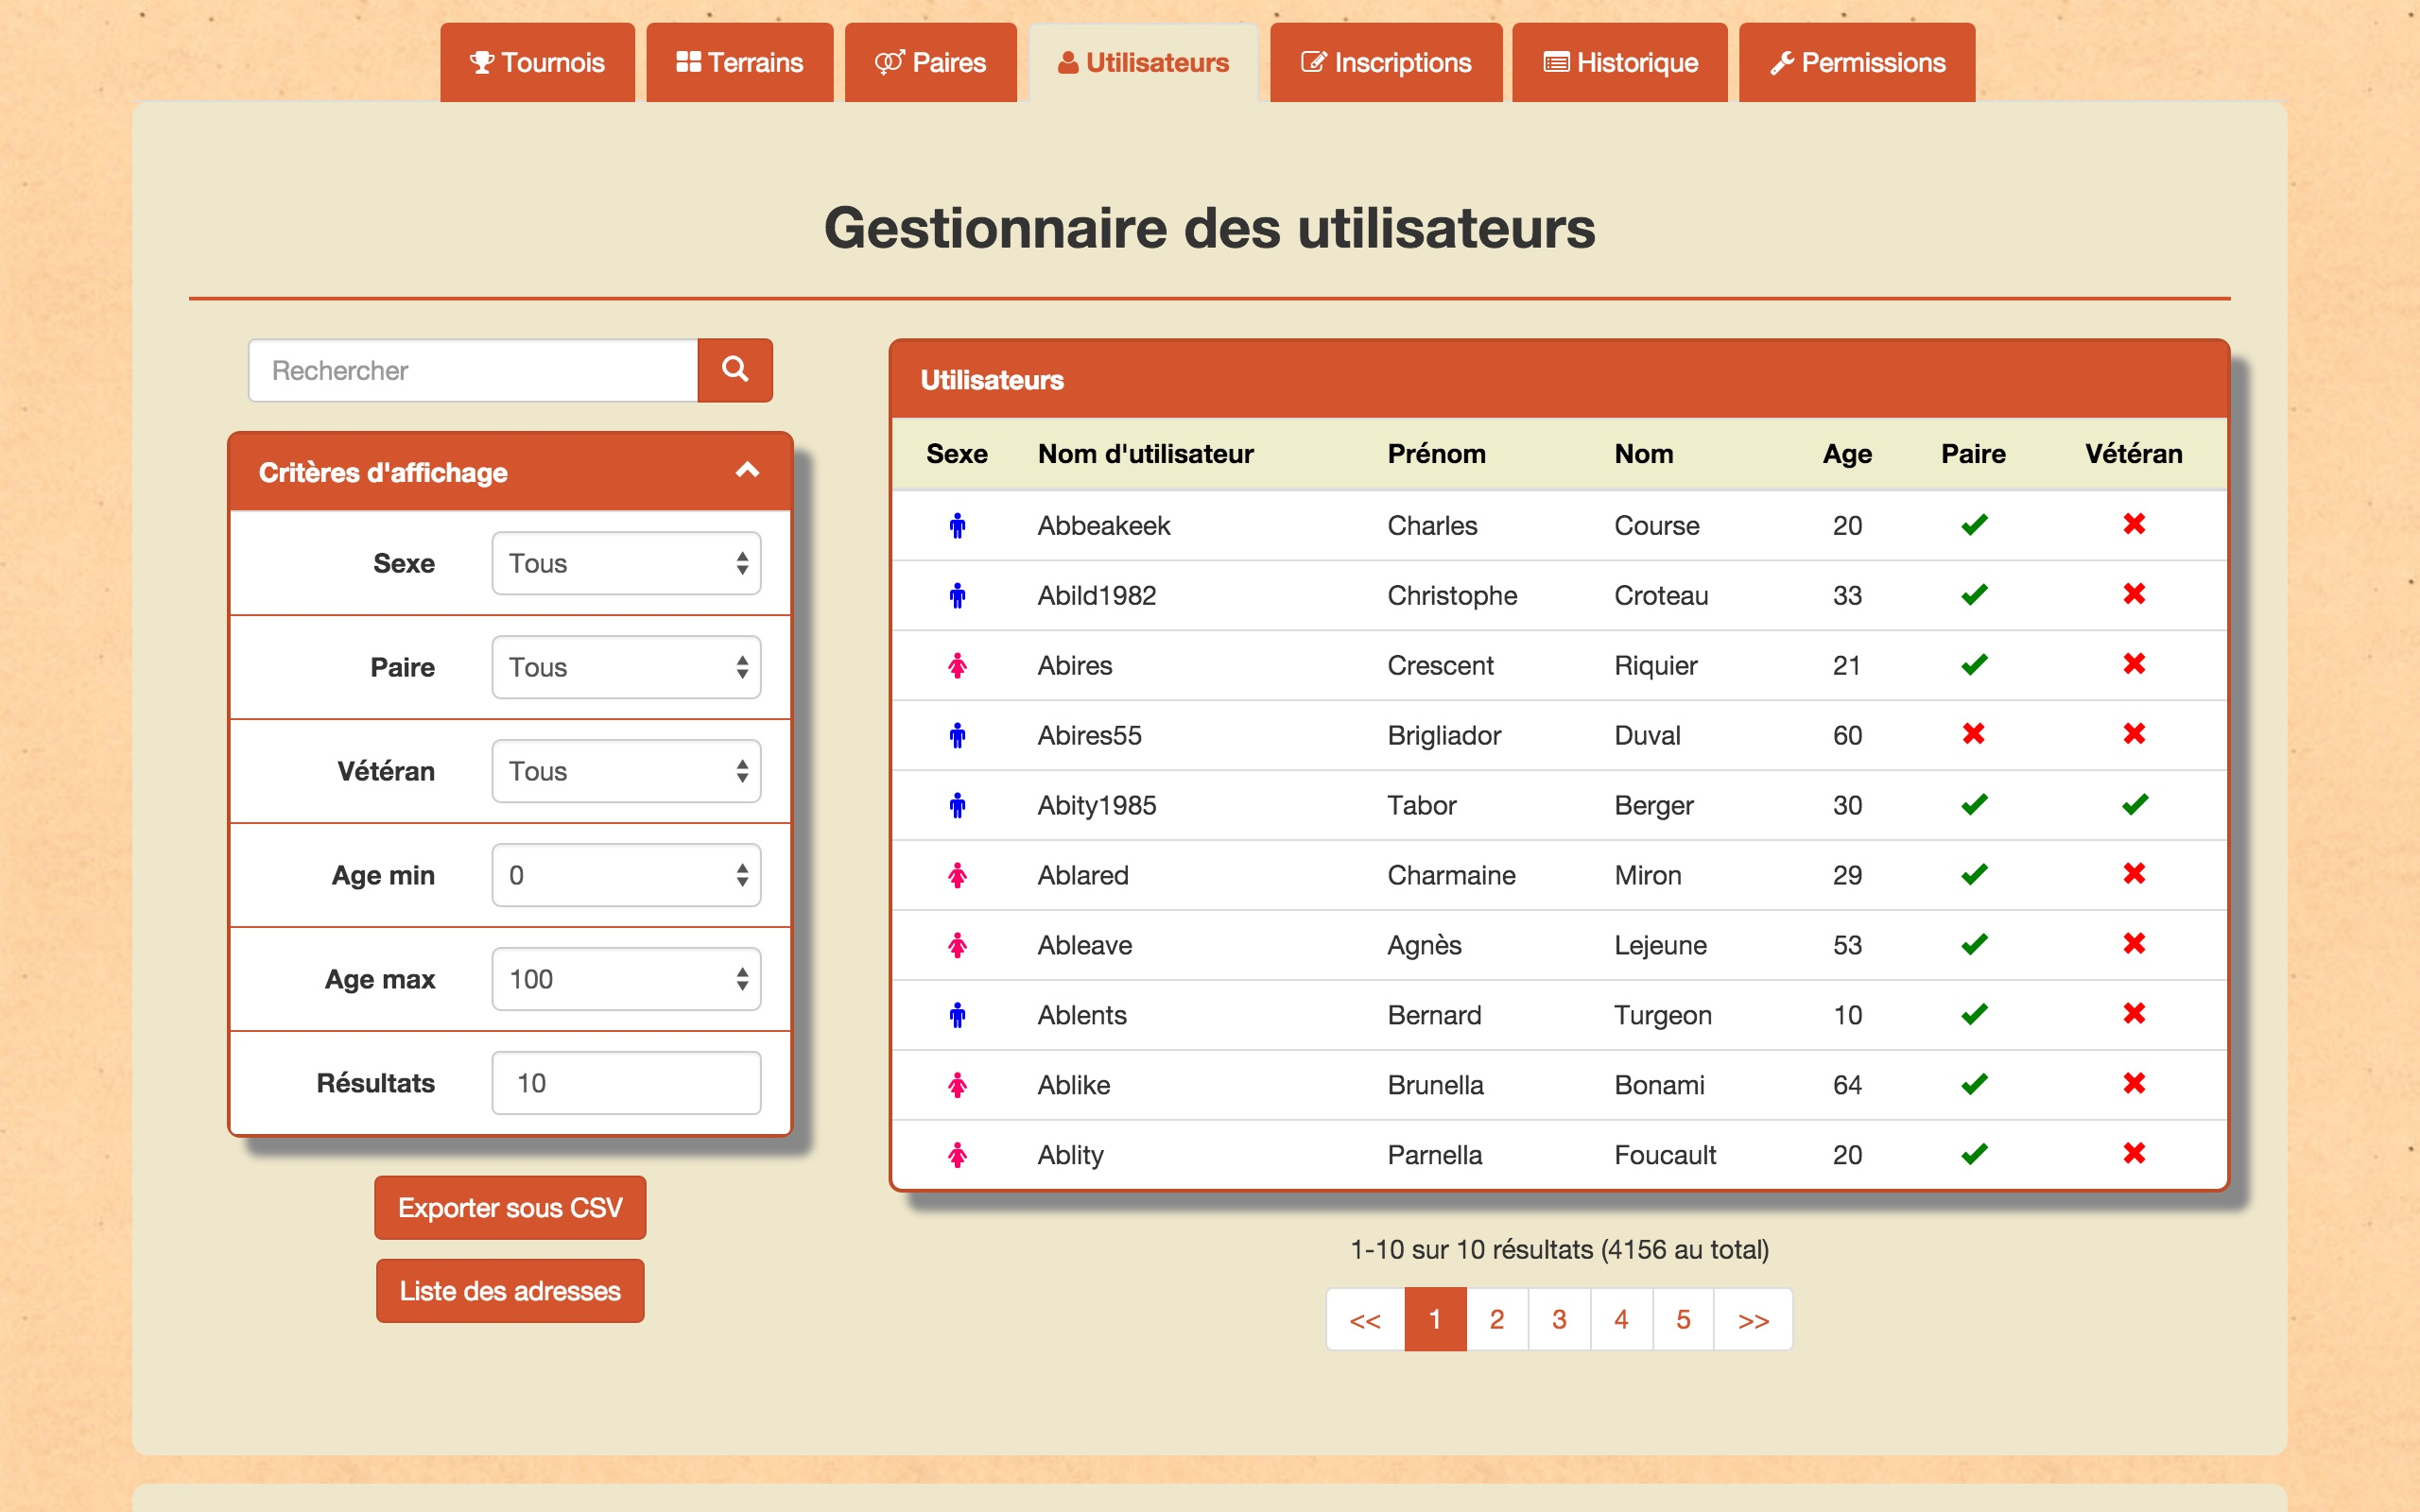
\includegraphics[scale=0.15]{gestion-users/gestion-users.jpg}
\caption{Page staff principale pour la gestion des utilisateurs}
\end{figure}

\subsection{Les utilisateurs}

Depuis la page staff \enquote{Gestionnaire des utilisateurs}, vous pouvez gérer tous les utilisateurs qui se trouvent dans la base de données. Pour donner la permission à un utilisateur de gérer les utilisateurs, l'admin doit lui octroyer les permissions à partir de la page enquote{Gestionnaire des permissions} \ref{Gestion des permissions}.\newline

Sur cette page, vous pouvez rechercher des utilisateurs, consulter un utilisateur, et l'éditer.\newline

La page principale de la gestion des utilisateurs est divisée en 2 parties :

\begin{itemize}
\item \textit{à gauche}, un champ et des critères de recherche, et deux boutons, l'un pour exporter la liste des utilisateurs au format CSV, l'autre pour télécharger uniquement la liste des adresses des utilisateurs ;
\item \textit{à droite}, la liste des utilisateurs qui respectent les critères choisies, et possédant certaines données qui ont une correspondance partielle avec le texte entré dans le champ de recherche ;
\end{itemize}
\bigskip

Les critères d'affichage des utilisateurs sont les suivants :

\begin{itemize}
\item \textbf{Sexe} permet de filter les utilisateurs selon leur sexe ;
\item \textbf{Paire} permet de filter les utilisateurs qui sont dans une paire ou non ;
\item \textbf{Vétéran} permet de filter les utilisateurs qui sont inscrits depuis plus d'une année ;
\item \textbf{Age min} permet de filter les utilisateurs dont l'âge est égal ou supérieur à celui mentionné ;
\item \textbf{Age max} permet de filter les utilisateurs dont l'âge est inférieur ou égal à celui mentionné ;
\item \textbf{Résultats} permet d'indiquer le nombre d'utilisateurs à afficher à la fois par page dans la liste des utilisateurs à droite
\end{itemize}
\bigskip

Pour effectuer une recherche, il faut sélectionner les critères et entrer le champ de recherche souhaité, puis valider la recherche en cliquant soit sur le bouton de la loupe, soit en appuyant sur la touche \textit{Entrée} du clavier. Le module des critères de recherche peut être minimisé, à tout moment, en cliquant sur le bouton dans le coin droit supérieur du module en forme de \enquote{V} (inversé si la liste des critères sont visibles).\newline

Pour consulter un utilisateur, il suffit de cliquer sur l'entrée de la liste des utilisateurs contenant les informations de l'utilisateur que l'on souhaite consulter. Par exemple, pour consulter l'utilisateur avec pour nom d'utilisateur \enquote{Abbeakeek}, il suffit de cliquer sur la ligne de la liste des utilisateurs où le texte \enquote{Abbeakeek} se trouve dans la colonne \enquote{Nom d'utilisateur}.

\subsection{Gestion d'un utilisateur}

\begin{figure}[H]
\centering
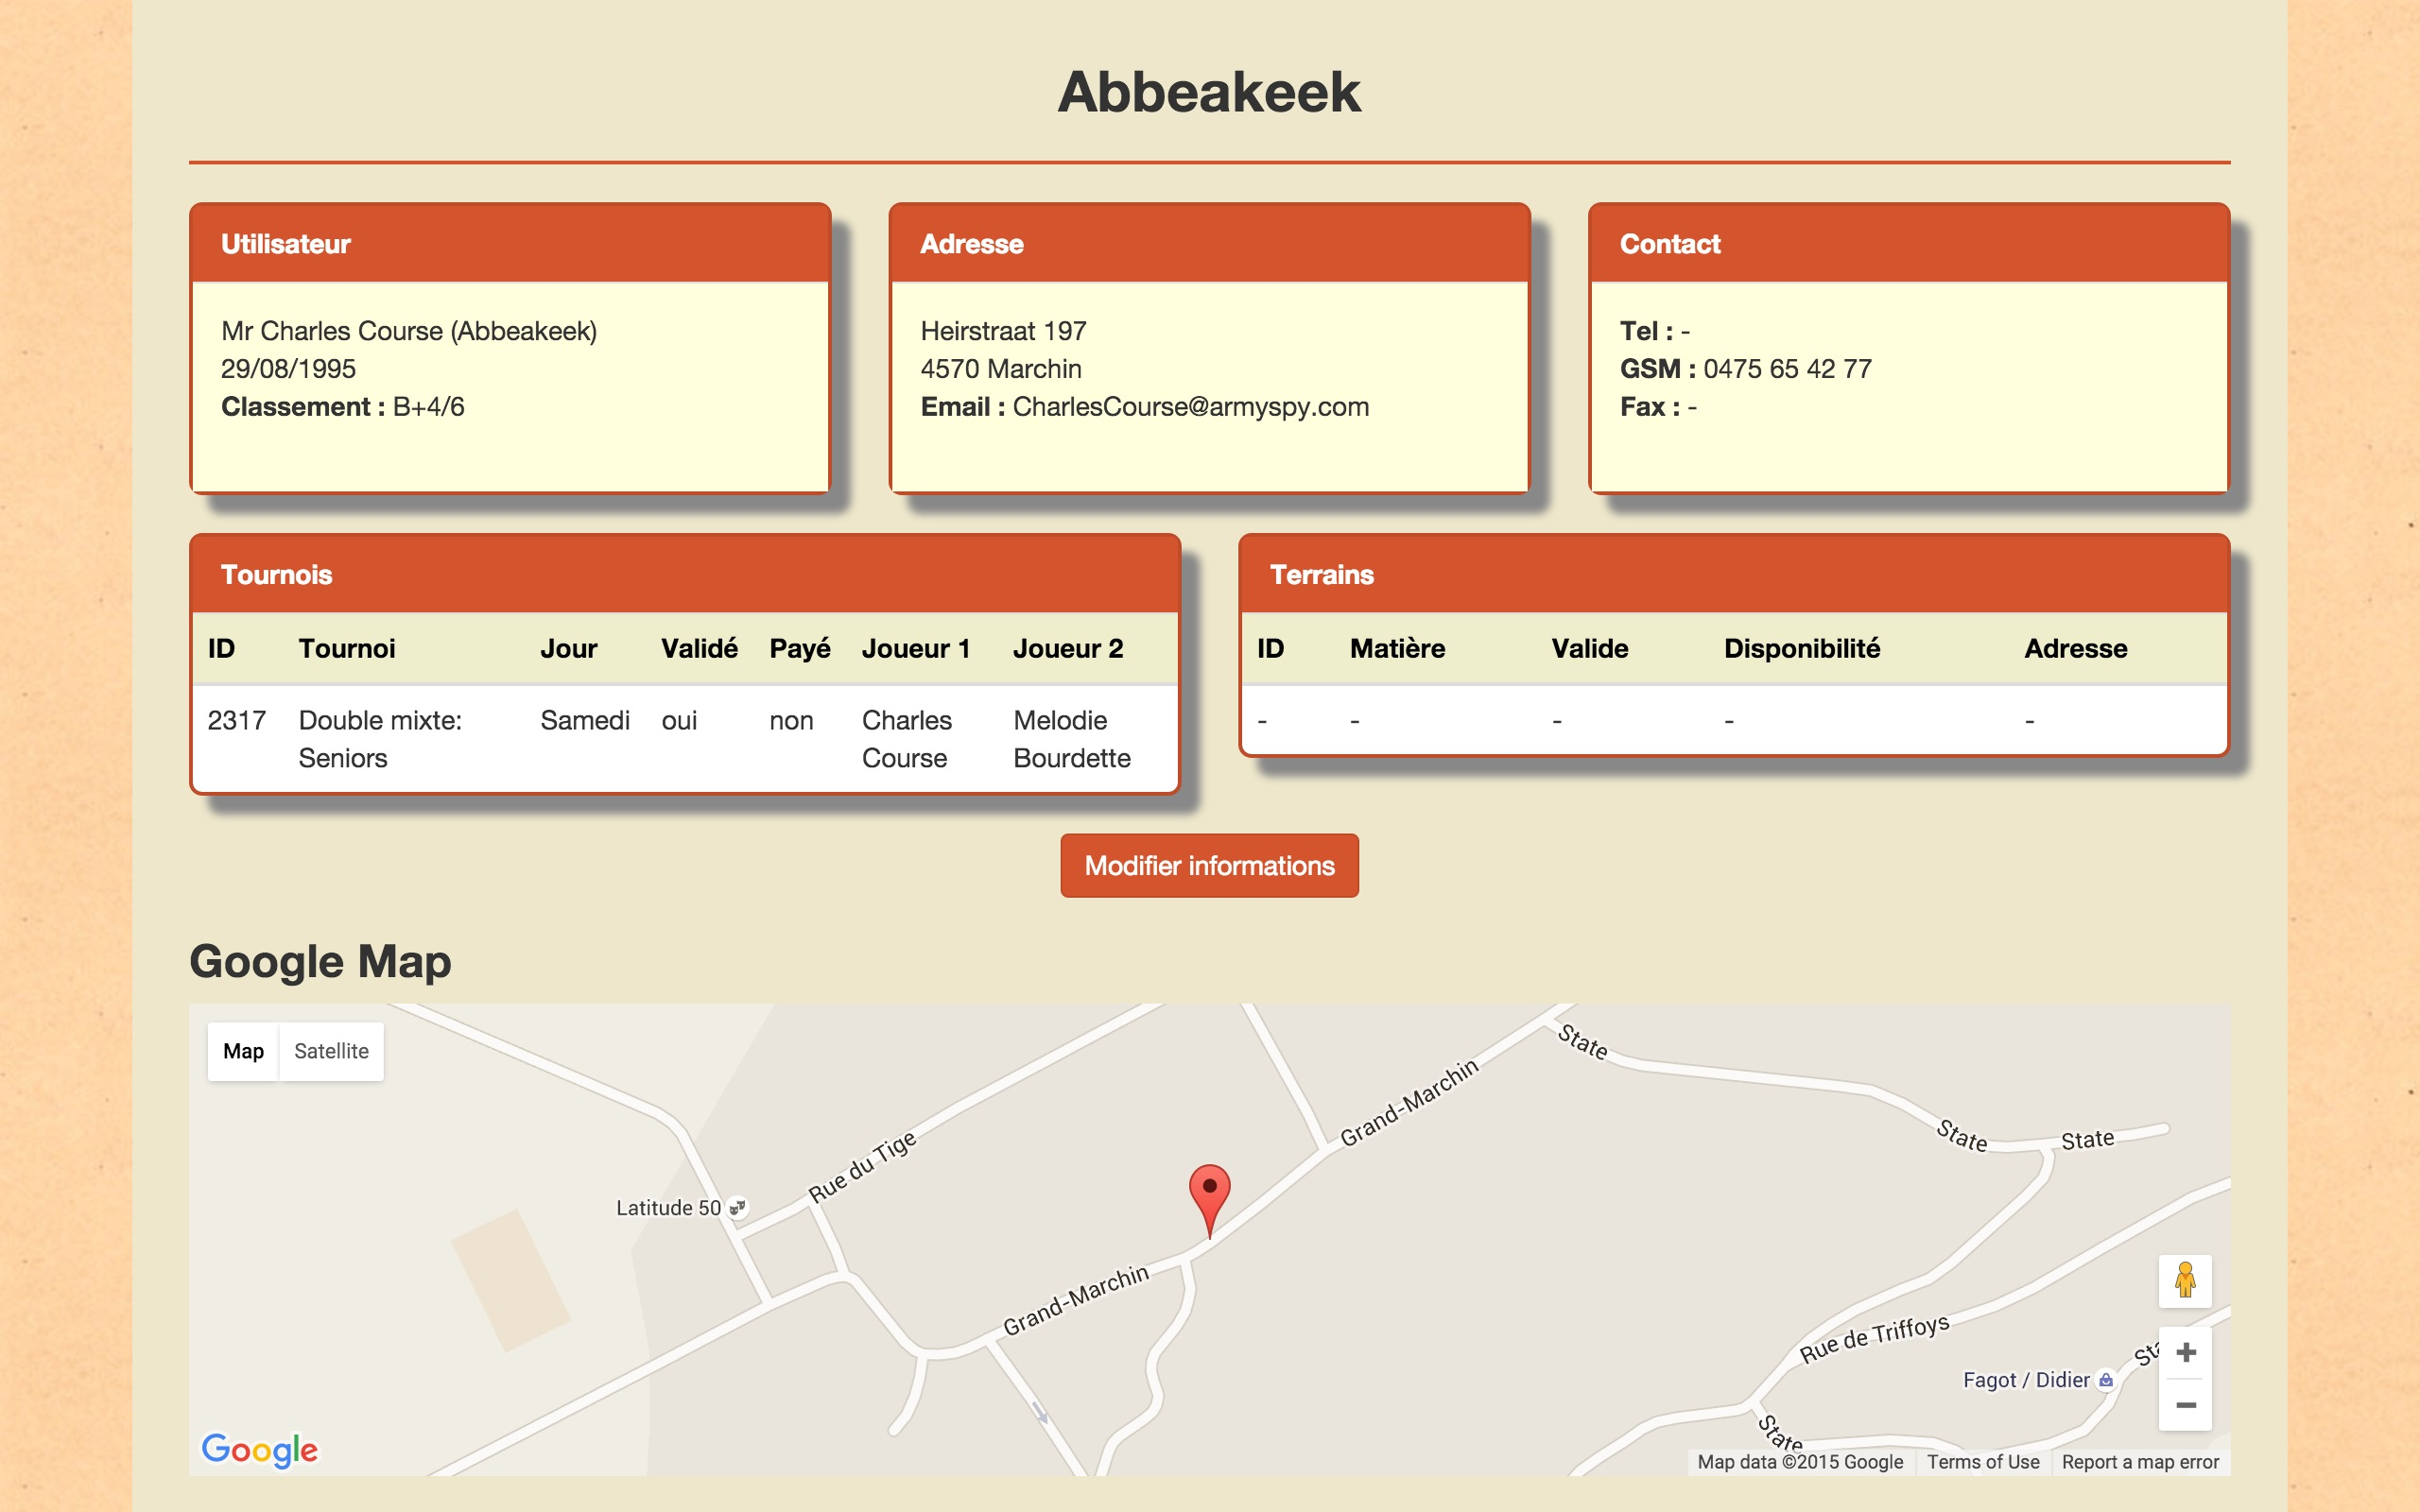
\includegraphics[scale=0.15]{gestion-users/gestion-users-user.jpg}
\caption{Page staff de la gestion d'un utilisateur}
\end{figure}

La page de la gestion d'un utilisateur se présente en plusieurs modules :

\begin{itemize}
\item \textit{le module \enquote{Utilisateur}} contient le nom de l'utilisateur, son nom de compte, sa date de naissance, et son classement ;
\item \textit{le module \enquote{Adresse}} contient son adresse physique et adresse email ;
\item \textit{le module \enquote{Contact}} contient son numéro de téléphone fixe, mobile, et fax ;
\item \textit{le module \enquote{Tournois}} contient la liste des inscriptions de l'utilisateur, où chaque entrée de la liste résume les informations de la paire. En cliquant sur la paire, le membre du staff peut directement accéder à la page de gestion la paire, pour autant qu'il ou elle ait la permission d'y accéder ! ;
\item \textit{le module \enquote{Terrain}} contient la liste des terrains de l'utilisateur, où chaque entrée de la liste résume les informations du terrain. En cliquant sur le terrain, le membre du staff peut directement accéder à la page de gestion du terrain, pour autant qu'il ou elle ait la permission d'y accéder !
\end{itemize}
\bigskip

Pour modifier les informations propres à l'utilisateur, il suffit de cliquer sur le bouton \textit{Modifier informations} pour accéder à un formulaire d'édition des informations de l'utilisateur, sous forme d'une boîte de dialogue.

\begin{figure}[H]
\centering
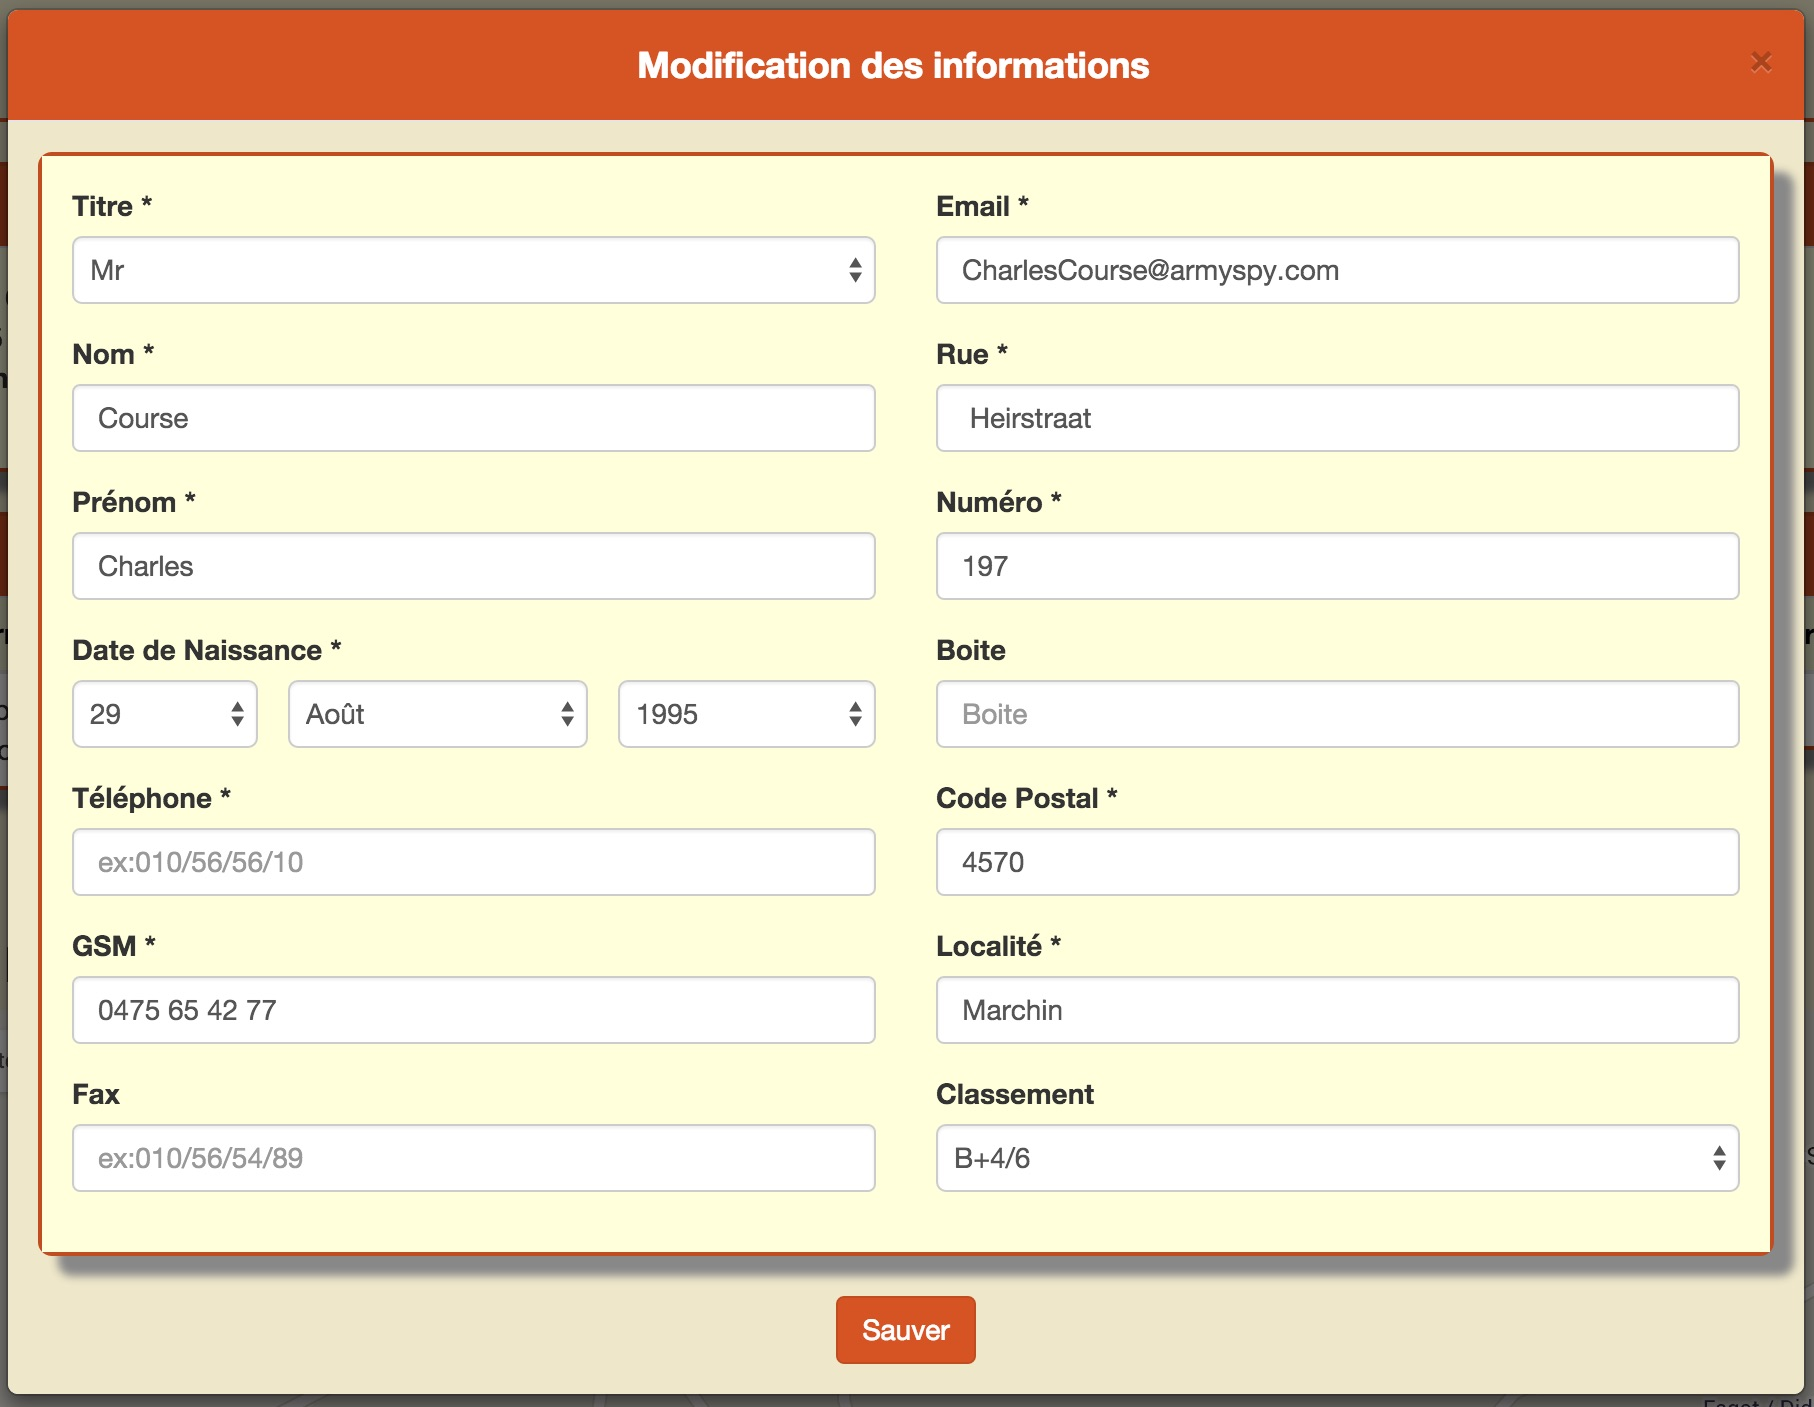
\includegraphics[scale=0.15]{gestion-users/gestion-users-edition.jpg}
\caption{Boîte de dialogue pour modifier les informations d'un utilisateur}
\end{figure}

Après avoir modifié les informations, il faut cliquer sur le bouton \textit{Sauver} pour appliquer les modifications. Pour annuler, il faut cliquer en dehors de la boîte de dialogue.